\chapter{Технологическая часть}

В данной части рассматриваются описываются выбранные средства реализации, структура классов программы, а также приводятся листинги реализации алгоритмов и приводится демонстрационный пример интерфейса программы.

\section{Средства реализации}
Для написания курсового проекта был выбран язык $C\#$\cite{}, предоставляющий достаточный набор инструментов для реализации спроектированного ПО. В частности, язык поддерживает объектно-ориентированную модель разработки, что позволяет выделять отдельные сущности задачи в виде классов.

В качестве интегрированной среды разработки была выбрана Microsoft Visual Studio 2022~\cite{}, предоставляющая достаточный функционал для написания, профилирования и отладки написанной программы, равно как и реализация пользовательского графического интерфейса ПО.

\section{Структура программы}
На рисунках~\ref{fig:SceneObjects}~-~\ref{fig:ClassDiagram} представлена диаграмма разработанных классов.
\begin{figure}[H]
	\centering
	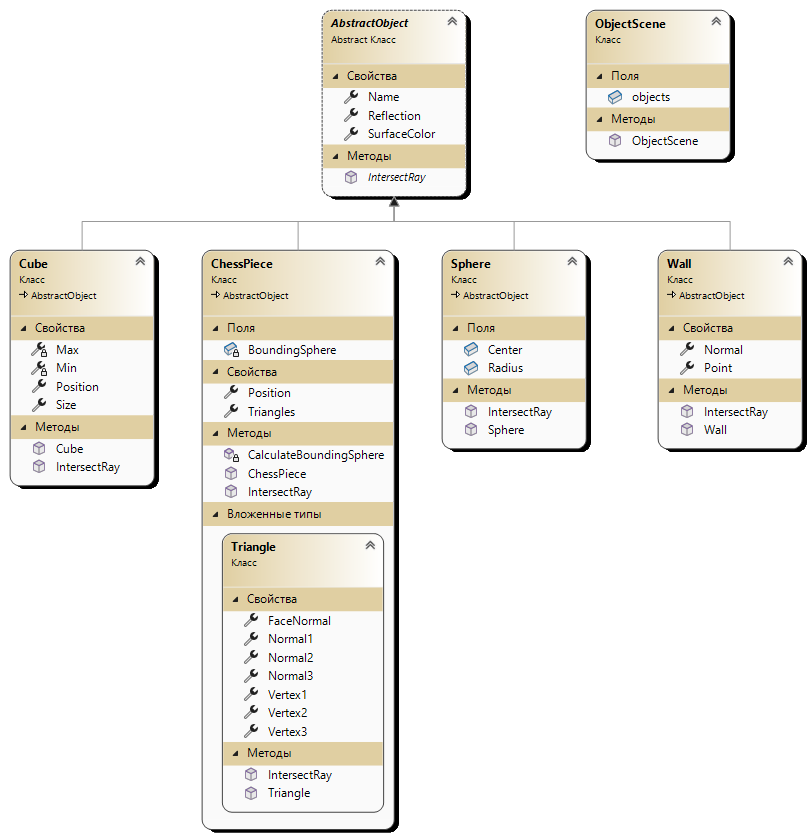
\includegraphics[width=0.6\textwidth]{objects_diagram}
	\caption{Диаграмма классов объектов сцены}
	\label{fig:SceneObjects}
\end{figure}

\begin{figure}[H]
	\centering
	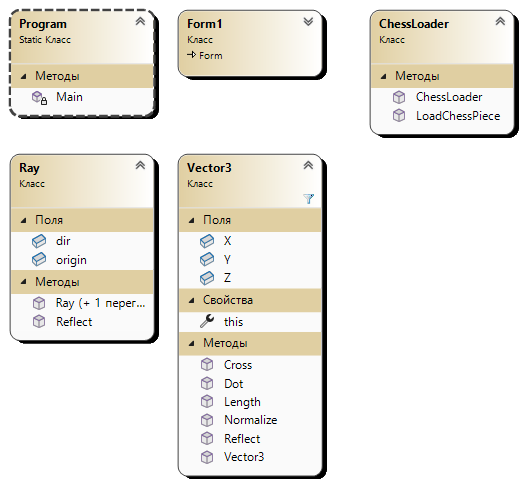
\includegraphics[width=0.4\textwidth]{ClassDiagram}
	\caption{Диаграммы вспомогательных классов}
	\label{fig:ClassDiagram}
\end{figure}

Разработанная программа состоит из следующих классов:
\begin{enumerate}
	\item структурные классы программы
	\begin{itemize}
		\item Program -- точка входа в программу;
		\item Form1 -- класс, представляющий графический интерфейс программы;
	\end{itemize}
	\item базовые математические классы
	\begin{itemize}
		\item Ray -- класс луча трассировки, также используется для представления камеры в программе;
		\item Vector3 -- класс трехмерного вектора, поддерживающий математические операции над векторами;
	\end{itemize}
	\item классы объектов сцены
	\begin{itemize}
		\item AbstractObject -- абстрактный класс, определяющий общий для всех объектов интерфейс;
		\item Cube -- класс, представляющий куб в качестве объекта сцены;
		\item ChessPiece -- класс, представляющий шахматную фигуру в качестве объекта сцены;
		\item Triangle -- класс для представления треугольных полигонов, из которых состоят шахматные фигуры;
		\item Sphere -- класс, представляющий сферу в качестве объекта сцены;
		\item Wall -- класс, представляющий стену в качестве объекта сцены;
	\end{itemize}
	\item ObjectScene -- класс, представляющий сцену объектов. Содержит список всех объектов сцены.
\end{enumerate}

\section{Реализация алгоритмов}
В соответствии со схемой, изображенной на рисунке~\ref{fig:RayTracing} был реализован алгоритм, приведенный на листинге~\ref{lst:RayTracing}.

\clearpage
\begin{center}
	\begin{lstlisting}[label={lst:RayTracing}, captionpos={b}, caption={Алгоритм трассировки лучей}]
	private Color TraceRay(Ray ray, ObjectScene scene, Vector3 lightPos, Color backgroundColor, int depth)
	{
		if (depth <= 0)
			return backgroundColor;
		
		double closestDistance = double.MaxValue;
		Vector3 hitNormal = new Vector3(0, 0, 0);
		AbstractObject closestObject = null;
		
		foreach (var obj in scene.objects)
		{
			if (obj.IntersectRay(ray, out double dist, out Vector3 normal) && dist < closestDistance)
			{
				closestDistance = dist;
				hitNormal = normal;
				closestObject = obj;
			}
		}
		
		if (closestObject == null)
			return backgroundColor;
		
		Vector3 hitPoint = ray.origin + ray.dir * closestDistance;
		Color objectColor = ((dynamic)closestObject).SurfaceColor;
		Color lightingColor = CalculateLighting(hitPoint, hitNormal, lightPos, objectColor, scene);
		
		if (closestObject.Reflection > 0)
		{
			Vector3 reflectionDir = ray.dir.Reflect(hitNormal);
			Color reflectionColor = TraceRay(new Ray(hitPoint, reflectionDir), scene, lightPos, backgroundColor, depth - 1);
			lightingColor = MixColors(lightingColor, reflectionColor, closestObject.Reflection);
		}
		return lightingColor;
	}
	\end{lstlisting}
\end{center}

\section{Вывод}


\clearpage
